\documentclass[11pt,french,table]{article}
\usepackage[french]{babel}
\usepackage[margin=1in,a4paper]{geometry}
\usepackage{multicol}

% Custom fonts. This package is only available with XeLaTex (pdflatex is a mess to deal with)
\usepackage{fontspec}
\setmainfont{GeneralSans}[
    Path = assets/fonts/,
    Extension = .otf,
    UprightFont = *-Regular,
    ItalicFont = *-Italic,
    BoldFont = *-Bold,
    BoldItalicFont = *-BoldItalic
]

% Custom titling
\usepackage{titling}
\usepackage{tcolorbox}

% Lipsum paragraphs
\usepackage{lipsum}

% Custom headers
\usepackage{fancyhdr}
\pagestyle{fancy}
\fancyhead[L]{\theauthor}
\fancyhead[C]{\itshape{\thetitle}}
\fancyhead[R]{\thedate}
\setlength{\headheight}{20pt}

% Default mathematical packages
\usepackage{amsmath}
\usepackage{amsfonts}

% Exercises environment and styling
\usepackage{amsthm}
\newtheoremstyle{exercice}%
    {3pt}% Space above
    {3pt}% Space below
    {\large}% Body font
    {}% Indent amount
    {\bfseries}% Theorem head font
    {.}% Punctuation after theorem heading
    {\newline}% Space after theorem heading
    {\thmname{#1}\thmnumber{ #2}\thmnote{: #3}}% Theorem head spec (can be left empty, meaning ‘normal’)
\theoremstyle{exercice}
\newtheorem{exercice}{Exercice}
\newtheoremstyle{corrigé}%
    {3pt}% Space above
    {3pt}% Space below
    {\large}% Body font
    {}% Indent amount
    {\bfseries}% Theorem head font
    {.}% Punctuation after theorem heading
    {\newline}% Space after theorem heading
    {\thmname{#1}\thmnumber{ #2}\thmnote{: #3}}% Theorem head spec (can be left empty, meaning ‘normal’)
\theoremstyle{corrigé}
\newtheorem{corrigé}{Corrigé}
% Graphics
\usepackage{graphicx}

\pretitle{\begin{center}\LARGE\bfseries}
\title{Analyse Avancée I - Corrigé III}
\posttitle{\par\end{center}}

\renewcommand{\maketitlehookb}{
\begin{center}

\includegraphics[width=2cm]{assets/imgs/S4S_logo.png}
\end{center}
}

\author{Students 4 Students}
\date{Septembre 2022}

\renewcommand{\maketitlehookd}{
\begin{center}
\begin{tcolorbox}[boxrule=0pt,frame empty,width=0.8\textwidth]
Les mathématiques sont une gymnastique de l'esprit et une préparation à la philosophie. 

\end{tcolorbox}
\scriptsize{Cette série vous est délivrée par Lounès, Louis et Till.} 
\end{center}
}

\begin{document}

\maketitle
\begin{corrigé}
Pour visualiser comment le rang $N_\epsilon$ varie en fonction de $\epsilon$, il faut trouver son expression. Par la définition de la limite on a que 
\begin{equation}
    |\frac{1}{n}|<\epsilon, \forall \epsilon>0, n\geq N_\epsilon
\end{equation}
Donc en isolant $n$ de cette expression, on trouve que $n\geq 1/\epsilon=N_\epsilon$. \\
Plotter ensuite cette expression et visualiser comment en diminuant la valeur de $\epsilon$ de $1$ à $0.00001$, le rang $N_\epsilon$ devient précis. Voire figure \ref{fig1} ci-dessous \\
\begin{figure}[h!]
    \centering
    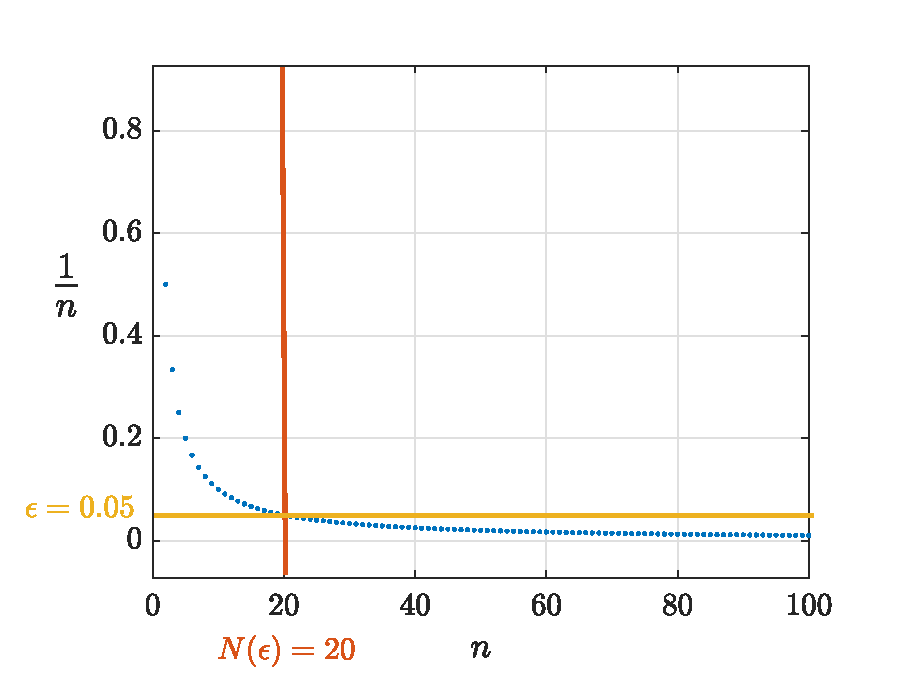
\includegraphics[width=90mm]{harmonique.eps}
    \caption{Suite $\frac{1}{n}$ et illustration de la convergence pour $\epsilon=0.05$.}
    \label{fig1}
\end{figure}
\end{corrigé}
\vspace{1em}
\begin{corrigé}
\begin{enumerate}
\item[]
    \item Faux. Prendre $u_n=n$ et $v_n=-n$. 
    \item Faux. Prendre $u_n=(-1)^n$ et $v_n=(-1)^n$. 
    \item Vrai. Par l'absurde, supposons que $(u_n+v_n)$ converge. Alors si on écrit 
    \begin{equation*}
        v_n=(u_n+v_n)-u_n,
    \end{equation*}
    $(v_n)$ converge comme somme de deux suites convergentes, ce qui est faux ! 
    \item Faux. Prendre $u_n=0$ et $v_n=n$. 
    \item Faux. Si l'on prend la suite $(u_n)$ définie telle que $U_{2n}=n$ et $u_{2n+1}=0$. Cette suite n'est pas majorée et ne tend pas vers $+\infty$ (car elle prend une infinité de fois la valeur zéro). 
    \item Faux. Si l'on prend la suite $(u_n)$ définie telle que $U_{2n}=1/n$ et $u_{2n+1}=2/n$ pour tout $n$ non nul. Alors $(u_n)$ tend vers $0$, est positive mais $u_{2n+1}>u_{2n}$ pour tout $n\geq 1$ et donc $(u_n)$ n'est pas décroissante à partir d'un certain rang $N$. 
\end{enumerate}
\end{corrigé}
\vspace{1em}
\begin{corrigé}
\begin{enumerate}
    \item [(a)] Vrai. juste un changement de notation (de $n$ à $k$).
    \item[(b)] Vrai. $\sum_{k=0}^{n} \frac{1}{n}=\frac{1}{n}+\frac{1}{n}+\frac{1}{n}+...+\frac{1}{n}=n*\frac{1}{n}=1$
    \item[(c)] Faux. $\sum_{k=1}^{n} \frac{1}{k}=1+\frac{1}{2}+\frac{1}{3}+...+\frac{1}{n}>1$
    \item[(d)] Vrai. $\sum_{k=0}^{n}x_n=x_0+x_1+x_2+x_3+...+x_n=x_{1-1}+x_{2-1}+x_{3-1}+...+x_{(n+1)-1}$
    \item[(e)] Vrai. $\sum_{k=0}^{100} k=0+1+2+3+4+5...+100=\frac{100\times101}{2}=5050$
    \item[(f)] Faux. Prendre $x_n=\frac{1}{n}$, on a alors $\lim_{n\xrightarrow[] \infty}{\frac{1}{n}}=0$ mais $\sum_{n=1}^{\infty}\frac{1}{n}=\infty$
    \end{enumerate}
\end{corrigé}

\vspace{1em}
\begin{corrigé}
Rappelons que 
    \begin{center}\textit{Une suite réelle est convergente si et seulement si c’est une suite de Cauchy.}
    \end{center}
    Ici nous vous demandons de faire la première partie de la preuve. \\
    Une suite $(x_n)\subset \mathbb{R}$ est dite de Cauchy si 
    \begin{equation*}
        \forall \epsilon>0, \ \exists N_\epsilon\in \mathbb{N} \  \text{ tel que } \  n,m>N_\epsilon \implies |x_n-x_m|<\epsilon. 
    \end{equation*}
    Ce qui revient à écrire $\lim\limits_{n,m\to \infty}{|x_n-x_m|}=0$ ou $|x_n-x_m|\to 0$. 
      \paragraph{Démonstration}
   
\paragraph{}
Supposons que $(x_n)$ est une suite convergente et posons $l$ sa limite. Alors 
\begin{equation*}
    \forall \epsilon >0, \ \exists N_\epsilon \in \mathbb{N} \ \text{ tel que } \ n\geq N_\epsilon \implies |x_n-l|<\frac{\epsilon}{2}. 
\end{equation*}
Ainsi pour tout $n,m\geq N_\epsilon$, il vient que : \begin{equation*}
    |x_n-x_m|=|(x_n-l)-(x_m-l)|\leq |x_n-l|+|x_m-l|<\frac{\epsilon}{2}+\frac{\epsilon}{2}=\epsilon. 
\end{equation*}
\end{corrigé}
\vspace{1em}
\begin{corrigé}
\vspace{1em}
\textit{Discussion} Une première remarque est que, dès lors qu'on ne sait pas qu'une suite $(u_n)$ converge on ne peut pas écrire lim $u_n$, c'est un nombre qui n'est pas défini ! En fait l'égalité : 
\begin{equation*}
    \lim\limits_{n\to \infty}{(-1)^n+1/n}=\lim\limits_{n\to \infty}{(-1)^n}
\end{equation*}
n'a pas de sens ! Par contre on peut dire que comme la suite $1/n$ tend vers $0$ pour $n$ grand, la suite $u_n$ est convergente \textbf{si et seulement si} la suite $(-1)^n$ l'est. De plus dans le cas où elle est convergente, elles ont toutes les deux la même limite. \paragraph{}
On veut montrer que la suite $(u_n)$ n'est pas convergente. Supposons alors par l'absurde qu'elle soit convergente vers un $l$ réel. \\
Considérons maintenant les sous-suites $v_n=u_{2n}$ et $w_n=u_{2n+1}$ de $(u_n)$. On a que $v_n=1+1/2n\to 1$ et que $w_n = -1+1/(2n+1)\to -1$. Or on sait que si une suite est convergente alors toute ses sous-suites ont la même limite !! 
Par conséquent ici on a que $\lim v_n=1$ et $\lim w_n=-1$, donc $l=1$ et $l=-1$ ce qui est une contradiction ! Donc $(u_n)$ ne converge pas. 
\paragraph{}
Montrons que $u_n$ est bornée. On a que 
\begin{equation*}
    \begin{aligned}
        -1 &\leq (-1)^n\leq 1 \\
        0 & \leq 1/n \leq 1 \\
    \end{aligned}
    \end{equation*}
    Donc 
    \begin{equation*}
                -1 \leq u_n \leq 2
    \end{equation*}
donc $u_n$ est bornée. 
\paragraph{}
Ce qu'on doit retenir : Par le théorème de Bolzano-Weierstrass, on sait que si $(u_n)$ est bornée alors il existe une sous-suite de $(u_n)$ qui est convergente. Cependant cela n'affirme en rien que $(u_n)$ est convergente ! \\ 
$(u_n)$ peut donc diverger mais admettre des sous-suites convergentes ! 
\end{corrigé}
\vspace{1em}
\begin{corrigé}
\vspace{1em}
 Montrons que $(x_n)$ croissante et bornée supérieurement $\implies$ $(x_n)$ convergente (la démonstration de l’autre cas étant tout à fait analogue).\\
 
Puisque $(x_n)$ est bornée supérieurement, il existe $b = \sup\{x_n ; n \in \mathbb{N}\}$. 

Maintenant, par définition du supremum, on a que
\begin{equation*}
    \forall \epsilon >0, \exists \overset{\sim}{n} \ \text{ tel que } \ b-\epsilon \leq x_{\overset{\sim}{n}}\leq b.
\end{equation*}
Or on sait que  $(x_n)$ est croissante et donc \begin{equation*}
    b-\epsilon \leq x_{\overset{\sim}{n}}\leq x_{\overset{\sim}{n}+1}\leq \cdots \leq b,
\end{equation*}
et ainsi $\lim x_n=b=\sup\{x_n; n\in \mathbb{N}\}$. 
\end{corrigé}
\vspace{1em}
\begin{corrigé}
Puisqu'il y équivalence entre suite de Cauchy et suite convergente, il suffit de démontrer que la suite $(x_n)$ n'est pas une suite de Cauchy, c'est à dire 
\begin{equation*}
    \exists \epsilon >0, \forall N \in \mathbb{N}, \exists n,m >N \ \text{ \textbf{ et} } \ |x_n-x_m|>\epsilon.
\end{equation*}
En effet en prenant $\epsilon =1$, $n=2N$ et $m=2N+1$ on a que $|x_n-x_m|=2>1$, ce qui achève la démonstration. 
\end{corrigé}
\end{document}